\documentclass[tikz,convert={outfile=\jobname.svg}]{standalone}
\usetikzlibrary{bayesnet}
\begin{document}
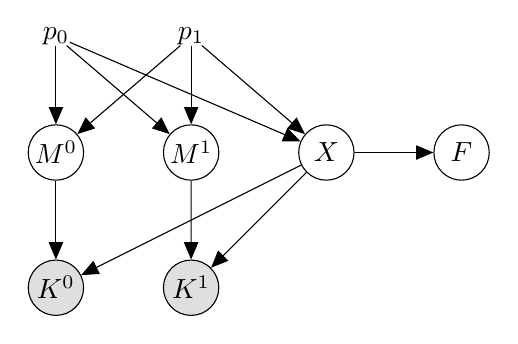
\begin{tikzpicture}
\node[style=latent](M0){$M^0$};
\node[style=latent, right=of M0](M1){$M^1$};
\node[style=latent, right=of M1](X){$X$};
\node[style=latent, right=of X](F){$F$};
\node[style=const, above=of M0](p0){$p_0$};
\node[style=const, above=of M1](p1){$p_1$};
\node[style=obs, below=of M0](K0){$K^0$};
\node[style=obs, below=of M1, right=of K0](K1){$K^1$};
\edge {p0,p1} {M0};
\edge {p0,p1} {M1};
\edge {p0,p1} {X};
\edge {X,M0} {K0};
\edge {X,M1} {K1};
\edge {X} {F};
\end{tikzpicture}
\end{document}
